\documentclass[11pt,letterpaper]{article}
\usepackage{fullpage}
\usepackage[top=0.5in, bottom=1.5in, left=1in, right=1in]{geometry}
\usepackage{amsmath,amsthm,amsfonts,amssymb,amscd}
\usepackage{lastpage}
\usepackage{enumerate}
\usepackage{enumitem}
\usepackage{fancyhdr}
\usepackage{graphicx}
\usepackage{listings}
\usepackage{hyperref}
\usepackage{booktabs}
\usepackage{cancel}
\usepackage{physics}
\usepackage{caption,cleveref,colortbl,csquotes,datatool,helvet,mathpazo,multirow,listings,pgfplots,xcolor}

\hypersetup{%
  colorlinks=true,
  linkcolor=blue,
  linkbordercolor={0 0 1}
}

\setlength{\parindent}{0.0in}
\setlength{\parskip}{0.05in}
\setlength{\footnotesep}{1.2\baselineskip}


% edit these
\newcommand\course{AST222H}
\newcommand\Title{Problem Set 2}
\newcommand\Name{Jeff Shen} 
\newcommand\Id{1004911526} 
\newcommand\Date{7 Feb 2020}

\pagestyle{fancyplain}
\headheight 35pt
\lhead{\Name}
\lhead{\Name\\\Id}
\chead{\LARGE \Title}
\rhead{\course \\ \Date}
\lfoot{}
\cfoot{}
\rfoot{\small\thepage}
\pgfplotsset{compat=1.16}
\headsep 1.2em

\begin{document}

% problem 1
\section*{Problem 1}
        The Oort constants $A$ and $B$ are 
        \begin{align*}
            A &= -\frac{1}{2}\left[\frac{d\Theta}{dR}\Big|_{R_0} - \frac{\Theta_0}{R_0}\right] \\
            B &= -\frac{1}{2}\left[\frac{d\Theta}{dR}\Big|_{R_0} + \frac{\Theta_0}{R_0}\right] \\
        \end{align*}
        Substituting in $\Theta(R) = \Theta_0 (R/R_0)^{-0.5}$, $A$ becomes 
        \begin{align*}
            A &= -\frac{1}{2}\left[\frac{d}{dR}\left(\Theta_0 - \sqrt{\frac{R_0}{R}}\right)\Big|_{R_0} - \frac{\Theta_0}{R_0}\right] \\ 
            &= -\frac{1}{2}\left[\Theta_0 \sqrt{R_0}\frac{d}{dR}\left(R^{-0.5}\right)\Big|_{R_0} - \frac{\Theta_0}{R_0}\right] \\ 
            &= -\frac{1}{2}\left[\Theta_0 \sqrt{R_0}\left(-\frac{1}{2}R^{-1.5}\right)\Big|_{R_0} - \frac{\Theta_0}{R_0}\right] \\
            &= -\frac{1}{2}\left[\Theta_0 \sqrt{R_0}\left(-\frac{1}{2}R_0^{-1.5}\right) - \frac{\Theta_0}{R_0}\right] \\
            &= -\frac{1}{2}\left[-\frac{1}{2}\frac{\Theta_0}{R_0} - \frac{\Theta_0}{R_0}\right] \\ 
            &= -\frac{1}{2}\left[-\frac{3}{2}\frac{\Theta_0}{R_0}\right] \\
            &= \frac{3}{4}\frac{\Theta_0}{R_0}.
        \end{align*}
        Following a similar procedure (with some steps omitted below) for $B$, we get 
        \begin{align*}
            B &= -\frac{1}{2}\left[\frac{d}{dR}\left(\Theta_0 - \sqrt{\frac{R_0}{R}}\right)\Big|_{R_0} - \frac{\Theta_0}{R_0}\right] \\ 
            &= -\frac{1}{2}\left[\Theta_0 \sqrt{R_0}\left(-\frac{1}{2}R_0^{-1.5}\right) + \frac{\Theta_0}{R_0}\right] \\
            &= -\frac{1}{2}\left[-\frac{1}{2}\frac{\Theta_0}{R_0} + \frac{\Theta_0}{R_0}\right] \\ 
            &= -\frac{1}{2}\left[\frac{1}{2}\frac{\Theta_0}{R_0}\right] \\
            &= -\frac{1}{4}\frac{\Theta_0}{R_0}.
        \end{align*}

        Taking $\Theta_0 = 220~{\rm km\,s^{-1}}$ and $R_0 = 8~{\rm kpc}$, we get the values 
        \begin{align*}
            A = 20.625~{\rm km\,s^{-1}\,kpc^{-1}} \qquad \text{and} \qquad B = -6.875~{\rm km\,s^{-1}\,kpc^{-1}}.
        \end{align*}
        Observed values are 
        \begin{align*}
            A = 15.3~{\rm km\,s^{-1}\,kpc^{-1}} \qquad \text{and} \qquad B = -11.9~{\rm km\,s^{-1}\,kpc^{-1}}.
        \end{align*}
        This shows that Keplerian rotation does not perfectly describe the rotation of the Milky Way near the Sun. 

% problem 2
\section*{Problem 2}
\begin{enumerate}[label=(\alph*)]
    \item The vertical position of the Sun is given by the equation 
        \begin{align}
            z(t) = A_Z\sin{(vt + \varphi)},
        \end{align}
        and the vertical velocity is given by its derivative with respect to time:
        \begin{alignat}{2}
            &&z'(t) &= A_Z\cos{(vt + \varphi)}v \nonumber\\
            \implies&&\frac{z'(t)}{v} &= A_Z\cos{(vt + \varphi)}.
        \end{alignat}
        Adding the squares of Eq. 1 and Eq. 2 give the following:
        \begin{align*}
            z(t)^2 + \left(\frac{z'(t)}{v}\right)^2 = A_Z^2\sin^2(x) + A_Z^2\cos^2(x) = A_Z^2(\sin^2(x) + \cos^2(x)) = A_Z^2.
        \end{align*}
        Using this to solve for $A_Z$, we get 
        \begin{align*}
            A_Z = \sqrt{z(t)^2 + \left(\frac{z'(t)}{v}\right)^2}.
        \end{align*}
        We know that at some $t=t_0$, we have $z(t_0) = 20~{\rm pc} = 6.171\times 10^{14}~{\rm km}$ and $z'(t_0) = 7.25~{\rm km\,s^{-1}}$. We also know that the vertical oscillation frequency $v$ is given by $v = \frac{2\pi}{p}$, where the period $p$ is equal to $85~{\rm Myr} = 2.68\times 10^{15}~{\rm s}$. Then, at $t=t_0$, $A_Z$ is given by 
        \begin{align*}
            A_Z = \sqrt{(6.171\times 10^{14}~{\rm km})^2 + \left(\frac{7.25~{\rm km\,s^{-1}}}{\frac{2\pi}{2.68\times 10^{15}~{\rm s}}}\right)^2} = 3.15\times 10^{15}~{\rm km} \simeq 102.2~{\rm pc}.
        \end{align*}
    \item The Sun's position oscillates radially with some amplitude $A_R$, given by 
        \begin{align*}
            A_R = \frac{9.16~{\rm kpc} - 7.92~{\rm kpc}}{2} = 0.62~{\rm kpc},
        \end{align*}
        about some average radial position $R_A$, given by 
        \begin{align*}
            R_A = \frac{9.16~{\rm kpc} + 7.92~{\rm kpc}}{2} = 8.54~{\rm kpc}.
        \end{align*}
        The radial position is given by 
        \begin{align*}
            r(t) = A_R\sin{(\kappa t)},
        \end{align*}
        and the velocity by its time derivative 
        \begin{align*}
            r'(t) = A_R\cos{(\kappa t)}\kappa.
        \end{align*}
        We know that at the current time $t=t_0$, the following is true:
        \begin{align*}
            r(t_0) = R_0 = A_R\sin{(\kappa t_0)}.
        \end{align*}
        Rearranging to solve for $t_0$, we find that 
        \begin{alignat*}{2}
            &&R_0 &= A_R\sin{(\kappa t_0)} \\
            \implies&&\frac{R_0}{A_R} &= \sin{(\kappa t_0)} \\
            \implies&&\kappa t_0 &= \arcsin{\left(\frac{R_0}{A_R}\right)} \\
            \implies&&t_0 &= \frac{\arcsin{\left(\frac{R_0}{A_R}\right)}}{\kappa}.
        \end{alignat*}

        \fbox{%
            \parbox{\linewidth}{%
                I didn't do it here, but it is probably better to skip the following step and to just compute $r'(t_0)$ from here. This ``avoids" the problem of having a negative time, and because the $\kappa$ term cancels out, some (annoying) conversions and rounding steps can be avoided. Doing this gives $r'(t_0) = 11.0~{\rm km\,s^{-1}}$.
            }
        }
        
        In this case, we take $R_0 = 8.0~{\rm kpc}$ relative to the midpoint of the radial oscillation, $R_A = 8.54~{\rm kpc}$. Thus, in the equation above, we use $R_0 = 8.0~{\rm kpc} - 8.54~{\rm kpc} = -0.54~{\rm kpc}$. Using this value, and $\kappa = 36~{\rm km\,s^{-1}\,kpc^{-1}}$, we find that the current time $t_0$ is
        \begin{align*}
            t_0 &= \frac{\arcsin{\left(\frac{R_0}{A_R}\right)}}{\kappa} \\
            &= \frac{\arcsin{\left(\frac{-0.54~{\rm kpc}}{0.62~{\rm kpc}}\right)}}{36~{\rm km\,s^{-1}\,kpc^{-1}}} \\
            &= -0.0294~{\rm kpc\,s^{-1}\,km^{-1}} \times \frac{3.068\times 10^{16}~{\rm km}}{{\rm kpc}} \\
            &= -9.01\times 10^{14}~{\rm s}.
        \end{align*}

        We can ignore the fact that the time is negative because this is simply an intermediate value that will be put into $\cos$, which, as an even function, satisfies $\cos(x) = \cos(-x)$.
        We can convert the units of the epicycle frequency $\kappa$ into seconds: $\kappa = 36~{\rm km\,s^{-1}\,kpc^{-1}} = 1.167\times 10^{-15}~{\rm s^{-1}}$. We can use this and the current time to calculate the current velocity in the radial direction:
        \begin{align*}
            r'(t_0) &= A_R\cos(\kappa t_0)\kappa \\
            &= 0.62~{\rm kpc}\times \cos(1.167\times 10^{-15}~{\rm s^{-1}}\times -9.01\times 10^{14}~{\rm s})\times 36~{\rm km\,s^{-1}\,kpc^{-1}} \\
            &= 11.1~{\rm km\,s^{-1}}.
        \end{align*}

\end{enumerate}


\newpage
% problem 3
\section*{Problem 4}
Some useful information:
\begin{itemize}
    \item $G = 6.67\times 10^{-11}~{\rm m^3\,kg^{-1}\,s^{-2}}$
    \item $1~{\rm pc} = 3.086\times 10^{16}~{\rm m}$
    \item $1~{\rm M_\odot} = 1.989\times 10^{30}~{\rm kg}$
\end{itemize}

\begin{enumerate}[label=(\alph*)]
    \item We equate gravitational acceleration with centripetal acceleration and solve for circular velocity: 
        \begin{alignat*}{2}
            &&\frac{GM_{BH}m}{R^2} &= \frac{mv_c^2}{R} \\
            \implies&&v_c^2 &= \frac{GM_{BH}}{R} \\
            \implies&&v_c &= \sqrt{\frac{GM_{BH}}{R}},
        \end{alignat*}
        where $M_{BH} = 4\times 10^{6}~{\rm M_\odot}$ is the mass of the black hole in solar masses, and $R$ is the distance from the black hole in parsecs. We can convert these to SI units, which will yield a velocity in meters per second. Then, we can divide the velocity by $1000$ to get a velocity in kilometers per second:
        \begin{align*}
            v_c(R)~{\rm [km\,s^{-1}]} &= \sqrt{\frac{G~{\rm [m^3\,kg^{-1}\,s^{-2}]}\times M_{BH}~{\rm [M_\odot]}\times 1.989\times 10^{30}~{\rm [kg\,M_\odot^{-1}]}}{R~{\rm [pc]}\times 3.086\times 10^{16}~{\rm [m\,pc^{-1}]}}} \times \frac{1~{\rm [km]}}{1000~{\rm [m]}} \simeq \frac{131}{\sqrt{R~{\rm [pc]}}}
        \end{align*}

    \item The density at some radius is given by $\rho(r) = \rho_0(\frac{r}{1~{\rm pc}})^{-1.9}$. We want to find $\rho_0$. The mass enclosed in a sphere with a radius of $R~{\rm pc}$ is 
        \begin{align*}
            M(<R~{\rm pc}) &= \int_0^{2\pi}\int_0^{\pi}\int_0^{r}\rho_0 (\frac{r}{1~{\rm pc}})^{-1.9}\,r^2 \sin{\theta}\,dr\,d\theta\,d\phi \\
            &= 4\pi\rho_0 \int_0^R r^{0.1}\,dr \\
            &= 4\pi\rho_0 \left(\frac{r^{1.1}}{1.1}\right)\big|_0^R \\
            &= \frac{4\pi\rho_0}{1.1}R^{1.1}.
        \end{align*}
        The mass enclosed has units of $M_\odot$ since $\rho_0$ has units of $M_\odot\,pc^{-3}$, and the volume integral gives units of $pc^{3}$. 

        At $R=1$, we know that the mass enclosed is same as the mass of the black hole, $4\times 10^{6}~{\rm M_\odot}$. We can use this information to solve for $\rho_0$:
        \begin{alignat*}{2}
            &&M(<1~{\rm pc}) &= \frac{4\pi\rho_0}{1.1}(1)^{1.1} = \frac{4\pi\rho_0}{1.1} = 4\times 10^{6}~{\rm M_\odot} \\
            \implies&&\rho_0 &= 4\times 10^{6}\times~{\rm M_\odot} \times \frac{1.1}{4\pi}~{\rm pc^{-3}} \simeq 3.5\times 10^5~{\rm M_\odot\,pc^{-3}}.
        \end{alignat*}

    \item This is similar to (a), but instead of using the mass of the black hole, we use the enclosed mass of the star cluster: 
        \begin{align*}
            v_c = \sqrt{\frac{GM_{enc}}{R}},
        \end{align*}
        where $M_{enc}$ is given by the following (omitting units in the intermediate steps, but masses are in solar masses and distances are in parsecs):
        \begin{align*}
            M_{enc}(R) &= \int_0^{2\pi}\int_0^{\pi}\int_0^{r}\,\rho_0 r^{-\alpha}\,r^2 \sin{\theta}\,dr\,d\theta\,d\phi \\
            &= 4\pi\rho_0 \int_0^R r^{2-\alpha}\,dr \\
            &= 4\pi\rho_0 \frac{1}{3-\alpha}(r^{3-\alpha})\big|_0^R \\
            &= \frac{4\pi\rho_0}{3-\alpha}R^{3-\alpha}~{\rm [M_\odot]}.
        \end{align*}
        So the velocity is given by 
        \begin{align*}
            v_c = \sqrt{\frac{G}{R}\frac{4\pi\rho_0 R^{3-\alpha}}{3-\alpha}}.
        \end{align*}
        Again, we need to ensure that the units are consistent, and we can do this by multiplying by some conversion factors:
        \begin{align*}
            v_c = \sqrt{\frac{G}{R\times 3.086\times 10^{16}}\frac{4\pi\rho_0 R^{3-\alpha}}{3-\alpha}\times 1.989\times 10^{30}} \times \frac{1}{1000},
        \end{align*}
        which gives circular velocity in kilometers per second.

    \item As before, circular velocity is given by 
        \begin{align*}
            v_c = \sqrt{\frac{GM}{R}}.
        \end{align*}
        Here, $M$ is the total mass enclosed, and $v_c$ is the velocity due to the entire enclosed mass. We can separate this mass term into the mass of the black hole, $M_{BH}$, and the enclosed mass of the stellar cluster, $M_{SC}$:
        \begin{align*}
            v_c = \sqrt{\frac{G}{R}(M_{BH}+M_{SC})}.
        \end{align*}
        Then, we can rewrite the component masses in terms of the velocities due to those masses:
        \begin{alignat*}{2}
            v_{BH} &= \sqrt{\frac{GM_{BH}}{R}} &\qquad v_{SC} &= \sqrt{\frac{GM_{SC}}{R}} \\
            \implies M_{BH} &= \frac{R}{G}v_{BH}^2 &\qquad M_{SC} &= \frac{R}{G}v_{SC}^2
        \end{alignat*}
        Substituting this into the previous expression, we find that 
        \begin{align*}
            v_c &= \sqrt{\frac{G}{R}(M_{BH}+M_{SC})} \\
            &= \sqrt{\frac{G}{R}\left(\frac{R}{G}v_{BH}^2+\frac{R}{G}v_{SC}^2\right)} \\
            &= \sqrt{v_{BH}^2 + v_{SC}^2}.
        \end{align*}

    \item \hfill\vspace{-0.4cm}
        \begin{figure*}[!htbp]
            \hspace{-3.cm}
            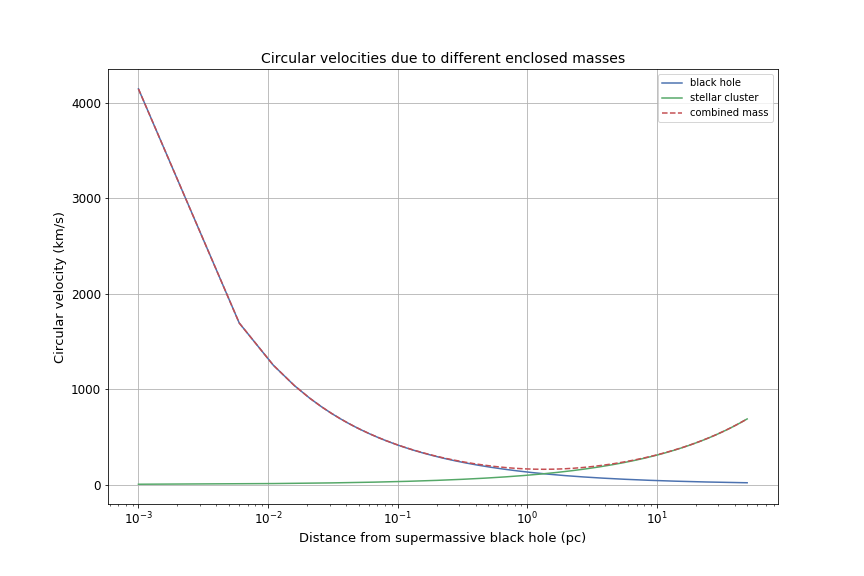
\includegraphics[width=1.4\linewidth]{velocity_curves.png}
        \end{figure*}

\end{enumerate}





\end{document}
